% begin module increasing-decreasing
\begin{frame}
\frametitle{Increasing and Decreasing Functions}
\begin{definition}[Increasing and Decreasing Functions]
A function $f$ is called increasing on an interval $I$ if $f(x_1) < f(x_2)$ whenever $x_1 < x_2$  in $I$.  

It is called decreasing on the interval $I$ if $f(x_1) > f(x_2)$ whenever $x_1 < x_2$ in $I$.
\end{definition}
\uncover<2->{
\begin{example}[Increasing and Decreasing]
\begin{columns}[t]
\column{.6\textwidth}
\ \only<-2>{%
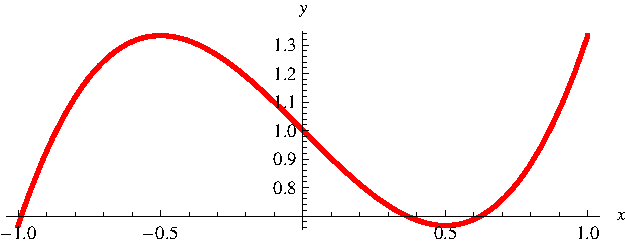
\includegraphics[height=2.8cm]{precalculus/pictures/01-01-inc-dec-a.pdf}%
}%
\only<handout:0| 3>{%
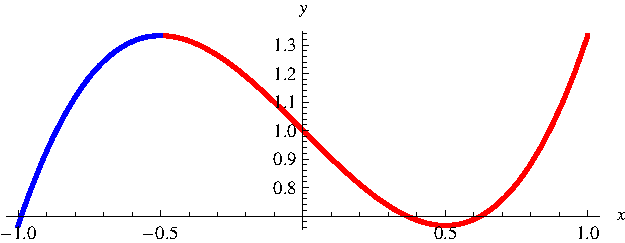
\includegraphics[height=2.8cm]{precalculus/pictures/01-01-inc-dec-b.pdf}%
}%
\only<handout:0| 4>{%
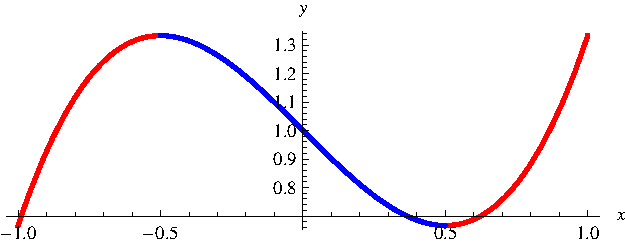
\includegraphics[height=2.8cm]{precalculus/pictures/01-01-inc-dec-c.pdf}%
}%
\only<handout:0| 5->{%
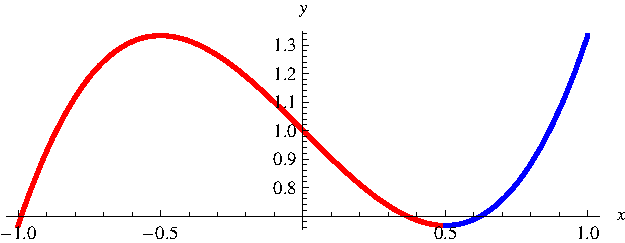
\includegraphics[height=2.8cm]{precalculus/pictures/01-01-inc-dec-d.pdf}%
}%
\column{.4\textwidth}
\begin{itemize}
\item<3-| alert@3>  $f$ is increasing on $[-1, -\frac{1}{2}]$.
\item<4-| alert@4>  $f$ is decreasing on $[-\frac{1}{2}, \frac{1}{2}]$.
\item<5-| alert@5>  $f$ is increasing on $[\frac{1}{2}, 1]$.
\end{itemize}
\end{columns}
\end{example}
}
\end{frame}
% end module increasing-decreasing
